\section{Radburny ``Burnie'' Cinders}

\begin{center}
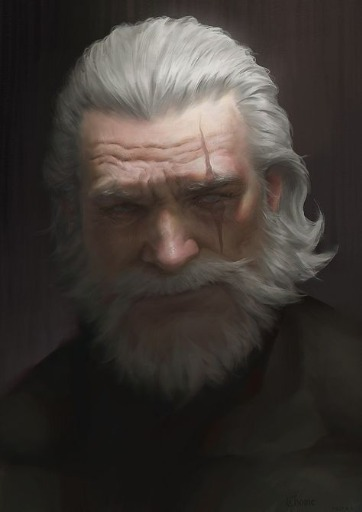
\includegraphics[width=80mm]{./content/img/burnie.png}
\begin{figure}[h]
\end{figure}
\end{center}

\subsection*{Details}

\noindent

Race: 	Human (Dwarf by adoption) \\
Class: 	Book Burner \\
Age: 	60 \\
Status: Active

\subsubsection{Background}

Radburny ``Burnie'' Cinders is a human raised by dwarven parents on a farm, who went on to become a Book Burner --- one of the Church's agents tasked with hunting down and destroying heretical texts.  Unlike many of his colleagues, Burnie survived the great Book Burner purges that destroyed the organisation, though the experience left deep scars.

Before joining the party, Burnie had a colourful career that included a stint at the University of Assassins, where he rose to a teaching position.  His personal life was equally eventful --- he fathered a child with Trayvon, a Tengu Book Burner colleague, producing a ``grossly disfigured'' half-human, half-Tengu son who grew up harbouring a deep hatred for his absent father.  The two eventually reconciled after the son attempted to kill Burnie, leading to ``a beautiful reconciliation'' where father and son ``quickly became best friends, making up for lost time''.

\subsubsection{Personality and Traits}

Burnie is a grouchy old man who is actually quite friendly underneath.  He has a talent for getting into trouble and an even greater talent for somehow surviving it.  His combat style is eclectic and unpredictable, wielding his sword Wasabi and whatever else comes to hand.

He has an unfortunate tendency to attract possession --- Mark O'Synne became trapped in his arm, trying to control his actions and prevent dangerous decisions.  Burnie's response to having a god lodged in his forearm was characteristically unfazed.

\subsubsection{Relationships}

Burnie has a son, known in academic circles as a Professor in Assassination Studies.  His adoptive dwarven parents still live on their farm and occasionally provide child-care services.

Within the party, Burnie formed a close bond with Kolo, the two sharing ``a little moment'' that hinted at genuine affection beneath the group's usual chaos.  He also developed a working relationship with his student Kevin, though this was widely described as ``unhealthily abusive''.  Martin the construct butler seems most attached to Burnie of all the party members.

\subsubsection{Burnie's Story}

Burnie joined the group after the departure of earlier companions, bringing his Book Burner expertise and grizzled determination to the cause.  His knowledge of the Church's inner workings and his connections to the remnants of the Book Burner network proved invaluable as the party navigated the political complexities of Hope's Rest and beyond.

During the expedition to the ancient dwarven mines, Burnie had a mysterious experience with a statue that left him looking ``flushed''.  He fought through giant spiders, cloakers, and a horrifying four-armed abomination in the depths, nearly dying when crushed in the creature's claw before being saved by Anthony Tigerius's berserker rage.

\clearpage
